\section{Sesión 4}
% SESSION V: Optimization IN ML

% For this session, the following tasks/questions need to be addressed:
% • Use the DFL scenario in Session I without attacks.
% • Run experiments with model optimization enabled using the following configurations.
% n Pruning
% § Apply structured pruning using l1_unstructured with an amount=0.8.
% n Quantization
% § Use precision="bf16-mixed" (to simulate training with reduced precision).
% • Track the following metrics during training:
% n Final F1 scores, model convergence, and round time.
% • Based on your experiments,
% n Which configuration provided the best trade-off between accuracy, efficiency, and
% convergence speed?

Compararemos la versión baseline de la sesión 1 con nuevas ejecuciones optimizadas con las técnicas
de \textit{pruning} y cuantización.

\vspace{1mm}

Mostramos la evolución del F1-score para los tres casos, viendo en el eje X el tiempo total de entrenamiento:

\vspace{1mm}

\noindent
\begin{minipage}{\textwidth}
    \centering
    \begin{tabular}{ccc}
        \textbf{Modelo baseline} & \textbf{Modelo con pruning} & \textbf{Modelo con cuantización} \\
        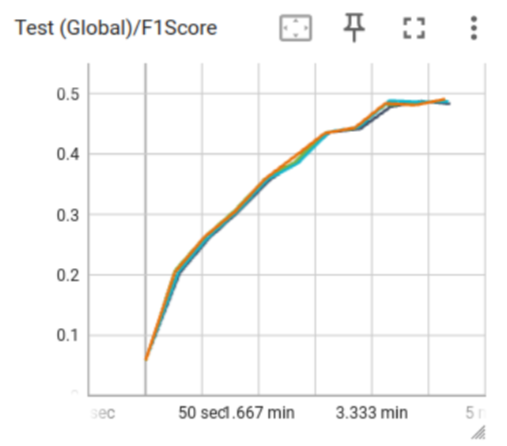
\includegraphics[width=0.25\textwidth]{images/baseline_f1_time.png} &
        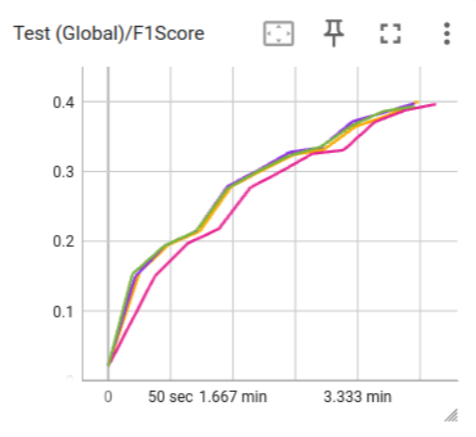
\includegraphics[width=0.25\textwidth]{images/pruning_f1_time.png}  &
        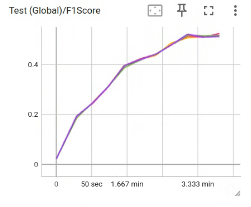
\includegraphics[width=0.25\textwidth]{images/quantization_f1_time.png} \\
    \end{tabular}
    \captionof{figure}{Impacto de técnicas de optimización en f1-score y tiempo de ejecución.}
    \label{fig:model_poisoning}
\end{minipage}
\vspace{1mm} 

Comparando el baseline con \textit{pruning}, vemos que claramente se ha degradado el rendimiento del modelo, pasando de un 0.48 de
F1-score a estar por debajo de 0.4. Esto se debe a que el modelo es más sencillo al tener menos información en sus pesos.
Sin embargo, no se ha reducido el tiempo total de entrenamiento, pues ambos tardan alrededor de 4 minutos y medio en completar 
las 10 rondas. El hecho de que no se mejore el tiempo creemos que se debe a que no se está utilizando ningún algoritmo
de compresión específico para tensores \textit{sparse} que permita aprovechar el pruning, por lo que al final se está mandando la misma
cantidad de datos por la red. 

\vspace{1mm}

Si comparamos el baseline con el modelo con cuantización vemos que sí se ha reducido el tiempo total de entrenamiento, 
pasando de 4 minutos y medio a 4 minutos. En cuanto al F1-score, no se ha degradado como sí ocurría en \textit{pruning},
manteniéndose por encima de 0.5 en todos los participantes.

\vspace{1mm}

Cabe destacar que en estos experimentos hemos forzado el uso de GPU cambiando una línea de código en \textit{nebula}, 
pues aunque nuestro ordenador con Linux nativo disponía de GPU, en los logs de entrenamiento especificaba que se estaba
usando CPU, por lo que la cuantización BF16 solo se estaba simulando y no obteníamos mejoras en tiempo. 

\vspace{1mm}

Esto se debía a que en la función \texttt{get\_available\_gpu} de \texttt{controller.py} solo se detectaba una GPU si 
su uso memoria tenía un uso por debajo al 5\%, lo que llevaba a descartar la GPU. Al subirlo al 50\% hemos visto en los
logs que sí está haciendo uso de esta. Este es el fragmento: 
\begin{verbatim}
    # Obtain available GPUs
    if memory\_used_percent < 50:
        available\_gpus.append(i)
\end{verbatim}

\subsection{Conclusión}
Podemos concluir que la optimización que mejores resultados ha obtenido en términos de precisión y eficiencia
(pues ha tardado menos tiempo en entrenar y ha obtenido mejor F1-score) ha sido cuantización, ya que al disponer
de GPU sí que aprovecha el uso de la técnica BF16 y conseguimos obtener una mejora real. Sin embargo, con \textit{pruning} 
no hemos conseguido una mejora real, al no disponer de un algoritmo de compresión en el envío de los pesos que se obtienen 
tras realizar el \textit{pruning}.

